\cleardoublepage
\section{Spezifikation OeVGK18}
\label{Spezifikation OeVGK18}

\subsection{Zusammenhang zur Berechnungsmethodik ARE}
\label{Spezifikation OeVGK18:Zusammenhang zur Berechnungsmethodik ARE}

In der Weisung des \acs{UVEK} vom 16.02.2015 ist festgehalten, dass für die Beurteilung der Qualität der Erschliessung mit dem öffentlichen Verkehr die \nameref{Lösungsansätze:Berechnungsmethodik ARE} verwendet wird~\cite{weisung_uvek}.
Dies ist der Grund warum im Folgenden der Bogen zu dieser Berechnungsmethodik geschlagen wird und die vorgeschlagenen Änderungen dieser Grundlagen gegenüber gestellt wird.
Die Berechnungsmethodik \acs{ARE} wird im Original~\cite{berechnung_are} zitiert und Anpassungen aus kantonalen Berechnungsmethodiken und eigene Verbesserungen werden, wo es Sinn macht, übernommen und gekennzeichnet.

\subsubsection{Art der Verkehrsmittel}
\label{Zusammenhang zur Berechnungsmethodik ARE:Art der Verkehrsmittel}

\begin{itquote}
Die Art der Verkehrsmittel, die an einer \gls{Haltestelle} abfahren, wird wie folgt unterschieden:
\begin{itemize}[noitemsep]
    \item Verkehrsmittelgruppe A
    \begin{itemize}
        \item Bahnknoten (mehrere Bahnlinien in verschiedenen Richtungen)
        \item Bahnlinien
    \end{itemize}
    \item Verkehrsmittelgruppe B
    \begin{itemize}
        \item Tram, Busse, Postautos, Rufbusse oder Schiffe
    \end{itemize}
    \item Verkehrsmittelgruppe C
    \begin{itemize}
        \item Seilbahnen
    \end{itemize}
\end{itemize}
\end{itquote}

Die Verkehrsmittel werden weiterhin in drei Gruppen gehalten.
Aufgrund der neuartigen Berechnung des Kursintervalls sind Bahnknoten und Bahnlinie in separaten Gruppen eingeteilt und Seilbahnen werden mit den restlichen Verkehrsmittel zusammen betrachtet.

\begin{itemize}[noitemsep]
    \item Verkehrsmittelgruppe A
    \begin{itemize}
        \item Bahnknoten
    \end{itemize}
    \item Verkehrsmittelgruppe B
    \begin{itemize}
        \item Bahnlinie
    \end{itemize}
    \item Verkehrsmittelgruppe C
    \begin{itemize}
        \item Tram, Bus, Postauto, Rufbus, Schiff, Seilbahn
    \end{itemize}
\end{itemize}

Als Bahnknoten gelten analog zu Berechnungsmethodik des Kanton Zürich Bahnstationen, die entweder einen Anschluss an den nationalen oder internationalen Fernverkehr haben und/oder Bahnlinien in mindestens 6 Richtungen verkehren. 

\subsubsection{Kursintervall}
\label{Zusammenhang zur Berechnungsmethodik ARE:Kursintervall}

\begin{itquote}
Als Stichtag für die Auswertung wird ein Werktag ausserhalb der Ferienzeit und der touristischen Hochsaison definiert.
\end{itquote}

Die Einschränkung zur Wahl des Stichtags wird übernommen.
Jedoch werden 2 weitere Zeiträume definiert, einer für das Wochenende und jeweils einer für die Nacht.

\begin{itquote}
Zur Berechnung des Kursintervalls an einer \gls{Haltestelle} werden aus dem elektronischen Fahrplan die Abfahrten auf allen Linien am Stichtag zwischen 6.00 und 20.00 Uhr gezählt.
Um die durchschnittliche Anzahl Abfahrten in eine Richtung zu ermitteln, wird die Anzahl Abfahrten halbiert.
Für Endhaltestellen sowie \glspl{Haltestelle}, die nur in einer Richtung befahren werden, erfolgen entsprechende Korrekturen.
Anschliessend wird das Kursintervall für die beiden Verkehrsmittelgruppen A und B separat berechnet (840 Minuten geteilt durch die korrigierte Anzahl Abfahrten).
\end{itquote}

Für die Kursintervallberechnung wird die statt der Anzahl Abfahrten die Wartezeit zwischen zwei Abfahrten als Grundlage verwendet.
Der Kursintervall $\tau$ einer \gls{Haltestelle} wird definiert als das "`Doppelte der erwarteten Wartezeit auf die nächste Abfahrt [\ldots] bei zufälligem Zugang im Zeitintervall $I = [a,b)$"'~\cite{visum_manual_formula}.

\subsubsection{Haltestellenkategorie}
\label{Zusammenhang zur Berechnungsmethodik ARE:Haltestellenkategorie}

\begin{itquote}
Die Haltestellenkategorie wird nach folgender Tabelle ermittelt:
\begin{table}[ht]
    \centering
    \begin{itquote}
    \begin{tabular}[c]{l | p{2.3cm} p{2.3cm} | p{2.2cm} | p{2.2cm}}
        \toprule
        \textbf{Kursintervall}
                                & \multicolumn{4}{c}{\textbf{Verkehrsmittelgruppe}}\\
        \midrule
        \textbf{}
                                & \multicolumn{2}{c|}{\textbf{A}}
                                & \multicolumn{1}{c}{\textbf{B}}
                                & \multicolumn{1}{c}{\textbf{C}}\\
        \textbf{}
                                & \textbf{Bahnknoten}
                                & \textbf{Bahnlinien}
                                & \textbf{Trams, Busse, Postautos, Rufbusse und Schiffe}
                                & \textbf{Seilbahnen}\\
        \textbf{< 5 min}
                                & I
                                & I
                                & II
                                & III\\
        \textbf{5 -- 9 min}
                                & I
                                & II
                                & III
                                & IV\\
        \textbf{10 -- 19 min}
                                & II
                                & III
                                & IV
                                & V\\
        \textbf{20 -- 39 min}
                                & III
                                & IV
                                & V
                                & V\\
        \textbf{40 -- 60 min}
                                & IV
                                & V
                                & V
                                & V\\
        \bottomrule
    \end{tabular}
    \end{itquote}
\end{table}
\end{itquote}

Bei der Gliederung des Kursintervalls wird die Einteilung der Berechnungsmethodik des Kanton Graubünden übernommen.
Dies führt zu einer feineren und erweiterten Gliederung des Kursintervalls und zwei zusätzlichen Haltestellenkategorien VI und VII.

\subsubsection{Distanz zur Haltestelle}
\label{Zusammenhang zur Berechnungsmethodik ARE:Distanz zur Haltestelle}

\begin{itquote}
Für die Distanz zur Haltestelle wird die Luftliniendistanz verwendet, d.h. die ÖV-Güteklassen bilden konzentrische Kreise um die Haltestelle.
Die Radien der Kreise betragen 300 m, 500 m, 750 m und 1‘000 m.
\end{itquote}

Als Einteilung werden neu Gehminuten mit der Einstufung 5, 7.5, 10 und 15 Minuten verwendet.
Unter der Annahme, dass die Laufgeschwindigkeit $1.4 m/s$ beträgt, wird die massgebende Gehdauer mithilfe der Laufgeschwindigkeit und der Anzahl zurückzulegende \gls{Leistungskilometer} berechnet, welche die Topographie und die Wegführung berücksichtigt.

\subsubsection{ÖV-Güteklassen}
\label{Zusammenhang zur Berechnungsmethodik ARE:ÖV-Güteklassen}

\begin{itquote}
Die Güteklassen werden nach folgender Tabelle ermittelt:
\begin{table}[ht]
    \centering
    \begin{itquote}
    \begin{tabular}[c]{l p{2.2cm} p{2.2cm} p{2.2cm} p{2.2cm}}
        \toprule
        \textbf{Haltestellenkategorie}
                                & \multicolumn{4}{c}{\textbf{Distanz zur \gls{Haltestelle}}}\\
        \midrule
        \textbf{}
                                & \textbf{< 300 m}
                                & \textbf{300 -- 500 m}
                                & \textbf{501 -- 750 m}
                                & \textbf{751 -- 1000m}\\
        \textbf{I}
                                & Klasse A
                                & Klasse A
                                & Klasse B
                                & Klasse C\\
        \textbf{II}
                                & Klasse A
                                & Klasse B
                                & Klasse C
                                & Klasse D\\
        \textbf{III}
                                & Klasse B
                                & Klasse C
                                & Klasse D
                                & keine\\
        \textbf{IV}
                                & Klasse C
                                & Klasse D
                                & keine
                                & keine\\
        \textbf{V}
                                & Klasse D
                                & keine
                                & keine
                                & keine\\
        \bottomrule
    \end{tabular}
    \end{itquote}
\end{table}
\end{itquote}

Durch die zusätzlichen Haltestellenkategorien VI und VII werden analog zur Berechnungsmethodik des Kanton Graubünden zwei weitere ÖV-Güteklassen E und F eingeführt.

\subsection{Berechnungsmethodik OeVGK18}
\label{Berechnungsmethodik OeVGK18}
Folgend wird die Berechnungsmethodik \gls{OeVGK18} detailliert beschrieben.
In Abbildung \ref{fig:Flow_OeVGK_Brechnung} ist zur Übersicht die Berechnung der \gls{ÖV-Güteklassen} schematisch dargestellt.
In einem ersten Schritt wird unter Berücksichtigung der Art der Verkehrsmittel (siehe Kapitel \ref{Berechnungsmethodik OeVGK18:Art der Verkehrsmittel}) und dem Kursintervall (siehe Kapitel \ref{Berechnungsmethodik OeVGK18:Kursintervall}) die Haltestellenkategorie (siehe Kapitel \ref{Berechnungsmethodik OeVGK18:Haltestellenkategorie}) eruiert.
Abschliessend werden mithilfe der Haltestellenkategorie und der Gehzeit zur \gls{Haltestelle} (siehe Kapitel \ref{Berechnungsmethodik OeVGK18:Gehzeit zur Haltestelle}) die ÖV-Güteklassen (siehe Kapitel \ref{Berechnungsmethodik OeVGK18:ÖV-Güteklassen}) berechnet.

\begin{figure}[ht]
    \centering
    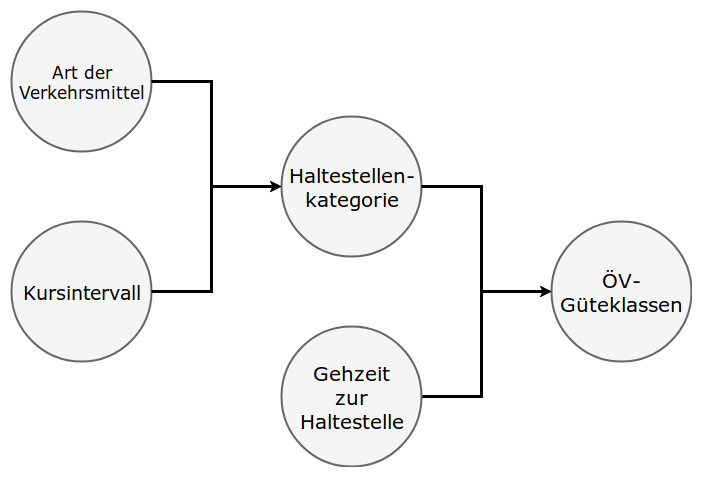
\includegraphics[width=0.7\linewidth]{technicalreport/img/Flow_OeVGK_Brechnung}
    \caption[Schema ÖV-Güteklassen Berechnung]{Schema ÖV-Güteklassen Berechnung}
    \label{fig:Flow_OeVGK_Brechnung}
\end{figure}

\subsubsection{Art der Verkehrsmittel}
\label{Berechnungsmethodik OeVGK18:Art der Verkehrsmittel}
Verkehrsmittel werden in folgende Verkehrsmittelgruppen eingeteilt:

\begin{itemize}[noitemsep]
    \item Verkehrsmittelgruppe A
    \begin{itemize}
        \item Bahnknoten
    \end{itemize}
    \item Verkehrsmittelgruppe B
    \begin{itemize}
        \item Bahnlinie
    \end{itemize}
    \item Verkehrsmittelgruppe C
    \begin{itemize}
        \item Tram, Bus, Postauto, Rufbus, Schiff, Seilbahn
    \end{itemize}
\end{itemize}

\paragraph{Bahnknoten}~\\
Bahnknoten sind Bahnstationen, die entweder einen Anschluss an den nationalen Fernverkehr haben und/oder Bahnlinien in mindestens 6 Richtungen verkehren.

Die Anzahl Richtungen einer Bahnstation wird gezählt als die Anzahl umliegender Bahnstationen, die mit einem beliebigen Zug innerhalb des definierten Zeitbereichs ohne Zwischenhalt erreicht werden können.

\paragraph{Schiffe und Seilbahnen}~\\
Schiffe und Seilbahnen werden nur berücksichtigt, wenn sie ein besiedeltes Wohngebiet erschliessen und nicht ausschliesslich für touristische Zwecke verwendet werden.


\subsubsection{Kursintervall}
\label{Berechnungsmethodik OeVGK18:Kursintervall}
Es sind 3 Stichtage mit jeweils zwei Zeitintervallen zu definieren, welche ausserhalb der Ferienzeit und der touristischen Hochsaison liegen.

\begin{table}[H]
    \centering
    \begin{tabular}[c]{l l}
        \toprule
        \textbf{Stichtag}
                                & \textbf{Zeitintervall}\\
        \midrule
        Werktag
                                & 06:00 -- 20:00 Uhr\\
        Werktag
                                & 20:00 -- 00:00 Uhr\\
        \midrule
        Samstag
                                & 06:00 -- 20:00 Uhr\\
        Samstag
                                & 01:00 -- 04:00 Uhr\\
        \midrule
        Sonntag
                                & 06:00 -- 20:00 Uhr\\
        Sonntag
                                & 01:00 -- 04:00 Uhr\\
        \bottomrule
    \end{tabular}
    \caption{Stichtag und Zeitintervall}
    \label{table:Stichtag und Zeitintervall}
\end{table}

Der Kursintervall $\tau$ einer \gls{Haltestelle} wird definiert als das "`Doppelte der erwarteten Wartezeit auf die nächste Abfahrt [\ldots] bei zufälligem Zugang im Zeitintervall $I = [a,b)$"'~\cite{visum_manual_formula}.
Es werden nur Abfahrten betrachtet, die innerhalb des definiertem Zeitintervall an der \gls{Haltestelle} abfahren.

Die Umsetzung dafür geschieht wie folgt:

\begin{tabbing}
Abfahrtszeitpunkte im Zeitintervall $I$: {\hskip 8em} \=    $x_{1 \ldots n}$      \\
Erste Abfahrt nach Zeitpunkt $b$ (nach Fahrplan): \>    $x'$                  \\
Fiktive Abfahrt nach $b$ bei zyklischer Fortsetzung: \> $x'' = x_1 + (b - a)$
\end{tabbing}

Für die Wartezeit am Zeitintervallende wird die Fahrt $x_{n+1} = min\{x', x''\}$ verwendet.

Kursintervall:
\[
    \tau^{a, b} = \frac{1}{b - a} \sum_{i=0}^n \Delta_i
\]

\begin{conditions}
    \Delta_i & $(x_{i+1} - x_i)^2$ {\hskip 2em} für $i \in \{1, \ldots, n - 1\}$ \\
    \Delta_0 & $(x_1 - a)^2$ \\
    \Delta_n & $(x_{n+1} - x_n)^2 - (x_{n+1} - b)^2$
\end{conditions}

\cleardoublepage
\subsubsection{Haltestellenkategorie}
\label{Berechnungsmethodik OeVGK18:Haltestellenkategorie}
Die Haltestellenkategorie I bis VII wird mit folgender Tabelle eruiert:

\begin{table}[H]
    \begin{tabular}[c]{l p{4.0cm} p{4.0cm} p{4.0cm}}
        \toprule
        \textbf{Kursintervall [min]}
                                & \multicolumn{3}{c}{\textbf{Verkehrsmittelgruppe}}\\
        \midrule
        \textbf{}
                                & \textbf{A}
                                & \textbf{B}
                                & \textbf{C}\\
        \textbf{≤ 5}
                                & I
                                & I
                                & II\\
        \textbf{(5, 10]}
                                & I
                                & II
                                & III\\
        \textbf{(10, 20]}
                                & II
                                & III
                                & IV\\
        \textbf{(20, 40]}
                                & III
                                & IV
                                & V\\
        \textbf{(40, 60]}
                                & IV
                                & V
                                & VI\\
        \textbf{> 60}
                                & -
                                & VII
                                & VII\\
        \bottomrule
    \end{tabular}
    \caption{Haltestellenkategorie}
    \label{Haltestellenkategorie}
\end{table}

\subsubsection{Gehzeit zur Haltestelle}
\label{Berechnungsmethodik OeVGK18:Gehzeit zur Haltestelle}
Bei der Berechnung der Gehzeit zu einer \gls{Haltestelle} ist eine Laufgeschwindigkeit von $1.4 m/s$ anzunehmen und die Strecke entlang des Wege- und Strassennetzes zu berücksichtigen, welche im Folgenden als Horizontaldistanz bezeichnet wird.

Damit man der Topographie gerecht wird, ist als massgebende zu laufende Distanz Leistungsmeter zu verwenden:
\[
    x = 
\begin{cases}
    a + b/0.1 + c/0.15, & \text{wenn } c/d>0.22\\
    a + b/0.1,          & \text{sonst}
\end{cases}
\]
\begin{conditions}
    x   &   Leistungsmeter [m]\\
    a   &   Horizontaldistanz [m]\\
    b   &   positive Steigung in Höhenmeter [m]\\
    c   &   negative Steigung in Höhenmeter [m]\\
    d   &   Horizontaldistanz mit negativer Steigung [m]
\end{conditions}

Die Gehzeit $t$ zur \gls{Haltestelle} ergibt sich nun aus:
\[ t = \frac{x}{1.4 m/s} \]


\subsubsection{ÖV-Güteklassen}
\label{Berechnungsmethodik OeVGK18:ÖV-Güteklassen}
Die Kombination aus Haltestellenkategorie und Gehzeit zur \gls{Haltestelle} liefert folgende \gls{ÖV-Güteklassen}-Gruppierung:

\begin{table}[H]
    \begin{tabular}[c]{l p{2.6cm} p{2.6cm} p{2.6cm} p{2.6cm}}
        \toprule
        \textbf{Haltestellenkategorie}
                                & \multicolumn{4}{c}{\textbf{Gehzeit zur \gls{Haltestelle} [s]}}\\
        \midrule
        \textbf{}
                                & \textbf{≤ 300}
                                & \textbf{(300, 450]}
                                & \textbf{(450, 600]}
                                & \textbf{(600, 900]}\\
        \textbf{I}
                                & Klasse A
                                & Klasse A
                                & Klasse B
                                & Klasse C\\
        \textbf{II}
                                & Klasse A
                                & Klasse B
                                & Klasse C
                                & Klasse D\\
        \textbf{III}
                                & Klasse B
                                & Klasse C
                                & Klasse D
                                & Klasse E\\
        \textbf{IV}
                                & Klasse C
                                & Klasse D
                                & Klasse E
                                & -\\
        \textbf{V}
                                & Klasse D
                                & Klasse E
                                & -
                                & -\\
        \textbf{VI}
                                & Klasse E
                                & -
                                & -
                                & -\\
        \textbf{VII}
                                & Klasse F
                                & -
                                & -
                                & -\\                                
        \bottomrule
    \end{tabular}
    \caption{ÖV-Güteklassen}
    \label{table:ÖV-Güteklassen}
\end{table}

Die Grenze wird bei einem Angebot schlechter als Stundentakt und einem Einzugsgebiet von 300 Sekunden gezogen, da man bei einer weiteren Betrachtung nicht mehr von einer Erschliessung reden kann und so auch nicht ausgewiesen werden soll.
